\documentclass[12pt,a4paper]{report}

\usepackage[brazil]{babel}
\usepackage[utf8]{inputenc}

\usepackage{graphicx}

\title{Especificações do Projeto SIGEST}
\author{Taciano Morais Silva - tacianosilva@gmail.com}

\begin{document}

\maketitle
\listoffigures
\tableofcontents

\chapter{Introdução}

Texto de introdução para testar a citação \cite{morais04a}.

\section{Definição de Perfis}

No sistema teremos vários tipos de usuário e seus respectivos perfis.
Segue abaixo a lista de usuários do sistema e seus respecitivos perfis. 

\emph{Professor} - Entidade que representa o professor que pode assumir um dos
seguintes perfis:

\begin{itemize}
\item Coordenador de Curso
\item Coordenador de Estágio
\item Avaliador de Estágio
\item Orientador de Estágio
\end{itemize}

\emph{Administrador} - Entidade que representa o super usuário que pode
assumir um dos seguintes perfis:

\begin{itemize}
\item Administrador
\item Super Administrador
\end{itemize}

\chapter{Projeto Arquitetural}

\chapter{Modelo de Dados}

% Figura Modelo de Dados
\begin{figure}[!htb]
        \centering
        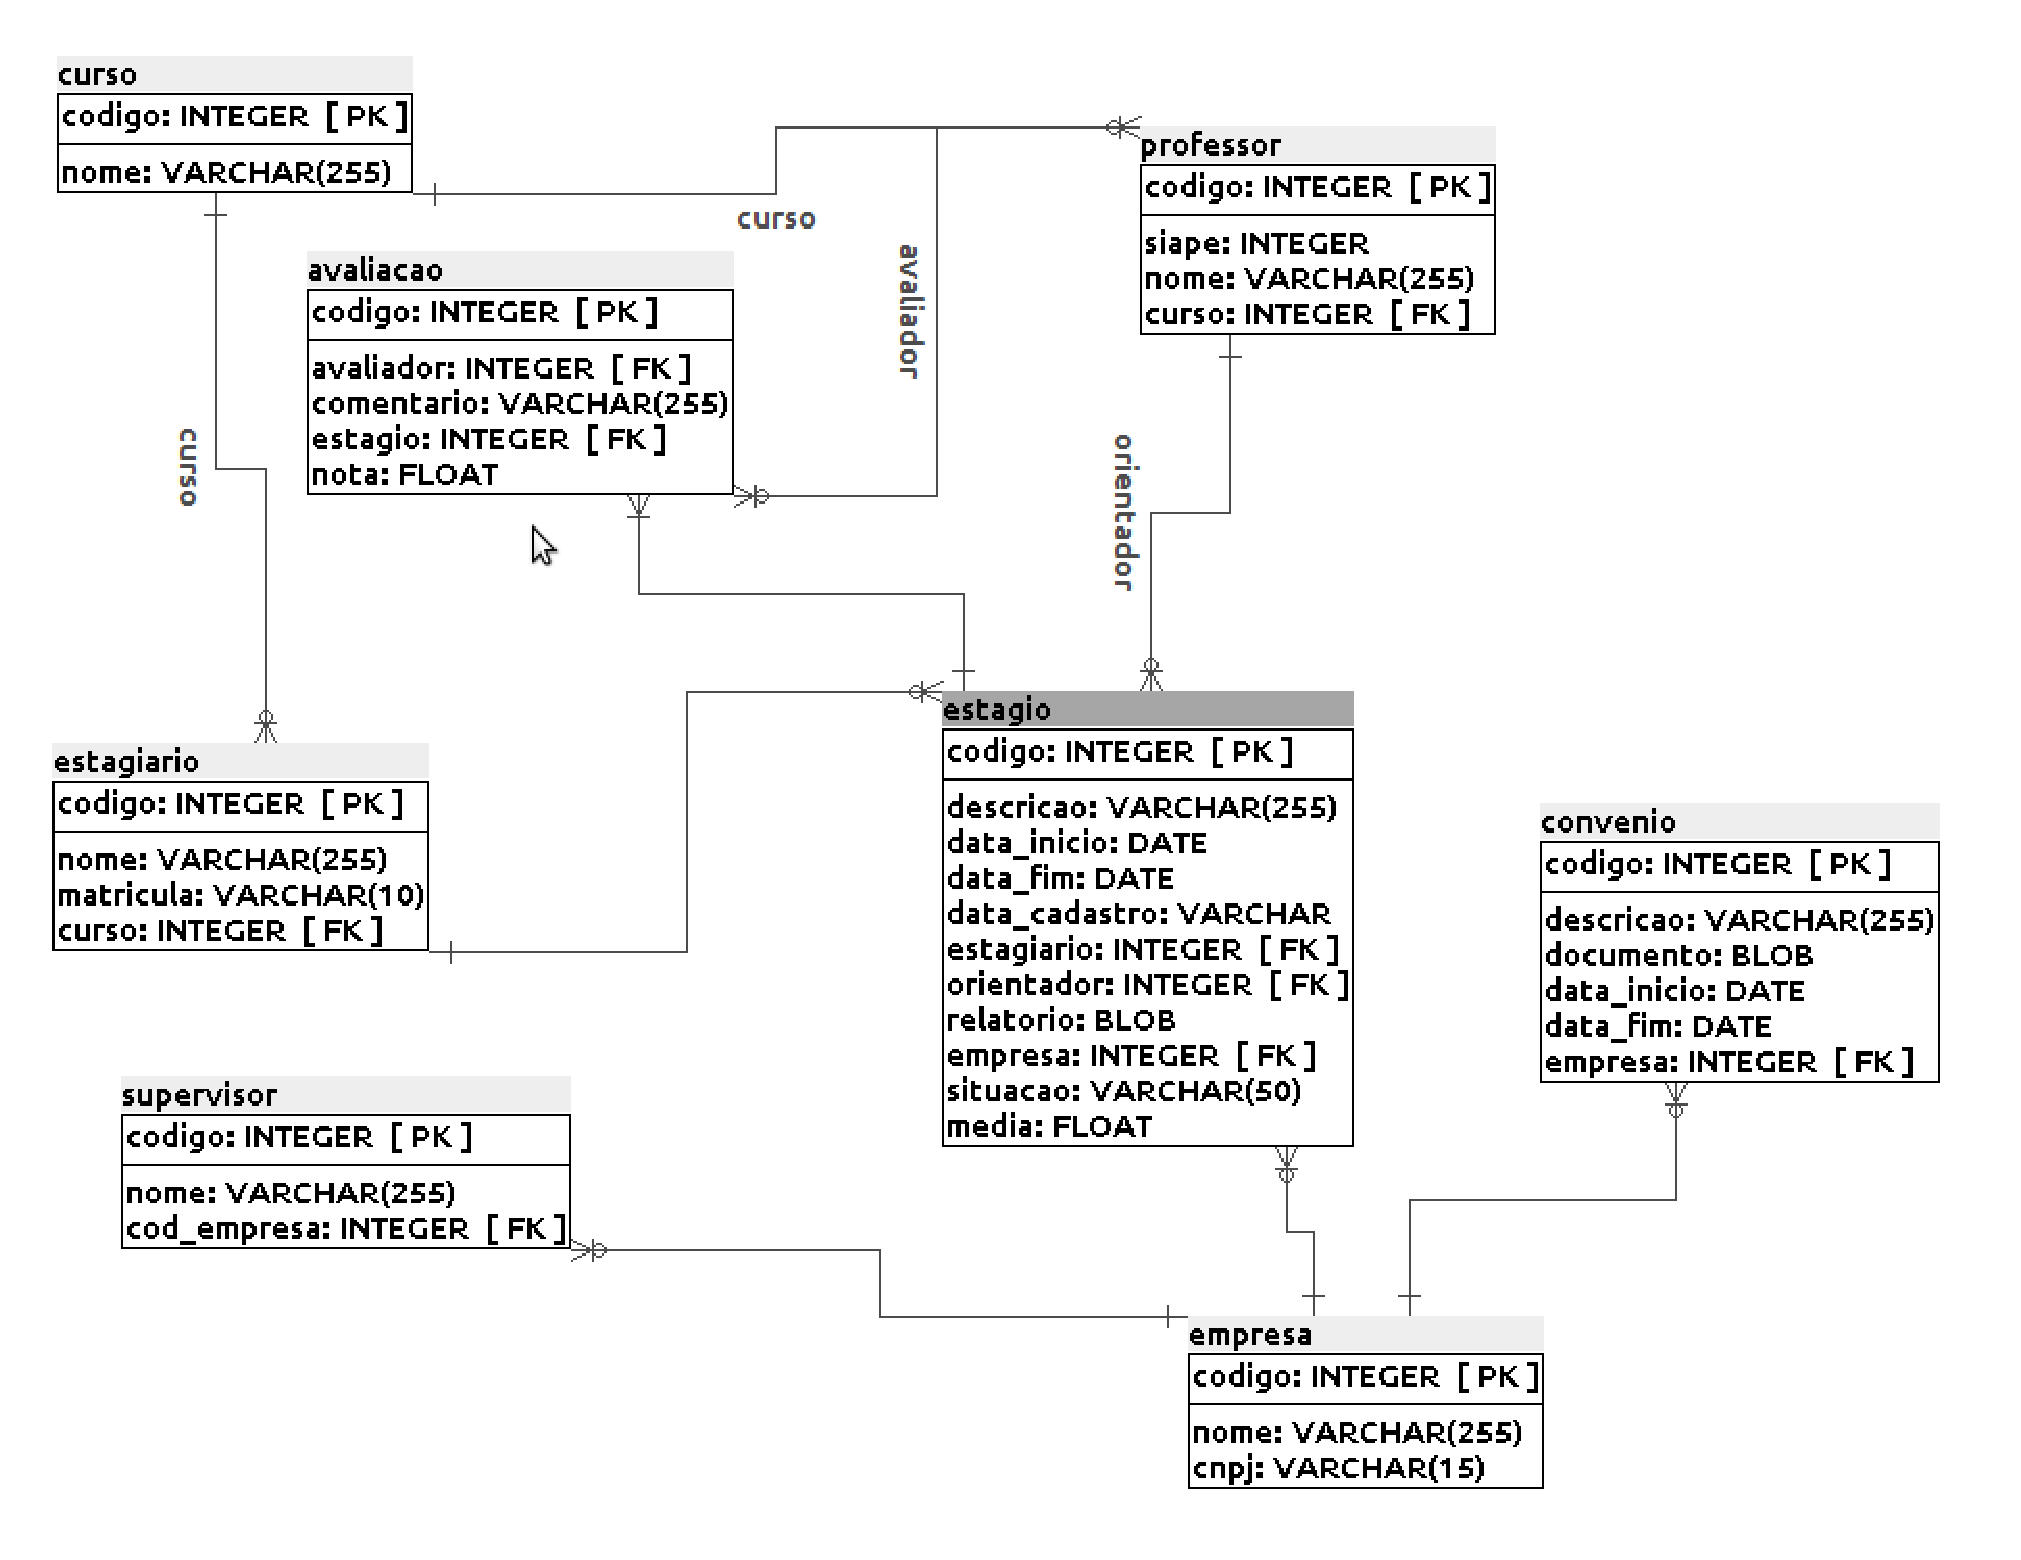
\includegraphics[scale=0.4]{esquema_sigest.eps}
        \caption{Esquema Relacionado para o Sistema SIGEST}
        \label{esquema_sigest}
\end{figure}
%\footnote{"A framework is a set of classes that embodies an abstract design for solutions to a family of related problems", \cite{johnson88}}


\chapter{Lista de Casos de Uso}

%% Input para a Section CDU001 - Estagiário
\section{CDU01 - Estagiário}

\subsection{Responsável}

Nome: Fladson

GitHub:

\begin{document}
\begin{tabular}{|p{4cm}|p{4cm}|p{4cm}|}
\hline
\textbf{Analista} &\textbf{Data Criação} &\textbf{Última Revisão}\\
\hline 
Jackson &$13\setminus03\setminus2013$ &\\
\hline
\end{tabular}

\section{Descrição}
O Caso de Uso Estagiário, será o responsável por conter as características e comportamentos
que um estagiário real possui quando está pagando a disciplina Estágio.

\subsection{Características de um Estagiário}
- Nome completo

- Matrícula

- Curso

\subsection{Relacionamentos de Estagiário com outras Entidades} 

- Empresa vinculada

- Coordenador de estágio

- Orientador de estágio

- Supervisor de estágio

- Data de submissão de proposta

- Nota final

\section{Pré-condição}
Para um estagiário ser cadastrado é necessário todos os seus dados serem preenchidos de
acordo com RN01 e RN04, e ter um curso anteriormente cadastrado de acordo com a RN02.

Para as funcionalidades “Alterar” e “Excluir”, a lei deverá ter sida já cadastrada no sistema,
de acordo com a RN03.

\section{Fluxos}

\subsection{Fluxo Principal}
\textbf{$[P1]$} O caso de uso se inicia quando o usuário abre o projeto WEB e aparece a tela de autenticação.

\textbf{$[P2]$} Ao Logar o usuário poderá selecionar a opção “Manter Estagiário”.

\textbf{$[P3]$} O usuário informa os dados necessários de acordo com o estagiário.

\textbf{$[P4]$} O usuário pressiona o botão “Incluir”, de acordo com as RN01, RN02, RN04.

\textbf{$[P5]$} Fim de caso de uso

\subsection{Fluxo Alternativo}

$[A1]$ O sistema exibe a mensagem (MS01) caso os campos obrigatórios não estejam preenchidos
corretamente ou completamente.

$[A2]$ O sistema exibe a mensagem (MS02) caso o numero da matrícula seja esteja cadastrado para
outro estagiário

$[A3]$ O usuário retorna para o passo P3 do FP.

\subsection{Excessões}

Não há excessões.

\section{Regras de Negócios Específicas}

$[RN01]$ Só poderá ser cadastrado o estagiário se todos os campos obrigatórios estiverem
preenchidos.

$[RN02]$ É necessário anteriormente possuir o curso referente ao mesmo cadastrado

$[RN03]$ Não é possível excluir um Estagiário ou alterá-lo sem que o mesmo esteja
cadastrado anteriormente.

$[RN04]$ O campo matrícula será único para cada cliente cadastrado.


\section{Mensagens do sistema}

$[MS01]$ – Preencha os campos obrigatórios.

$[MS02]$ – Matrícula já cadastrada, enforme outro número.

\section{Observações}

Não há Observações.

\end{document}


\section{CDU02 - Estágio}

\subsection{Responsável}

Nome: Aragon

GitHub:




<!DOCTYPE html>
<html>
  <head prefix="og: http://ogp.me/ns# fb: http://ogp.me/ns/fb# githubog: http://ogp.me/ns/fb/githubog#">
    <meta charset='utf-8'>
    <meta http-equiv="X-UA-Compatible" content="IE=edge">
        <title>sigest/docs/cdu002.tex at ramo_login · tacianosilva/sigest</title>
    <link rel="search" type="application/opensearchdescription+xml" href="/opensearch.xml" title="GitHub" />
    <link rel="fluid-icon" href="https://github.com/fluidicon.png" title="GitHub" />
    <link rel="apple-touch-icon" sizes="57x57" href="/apple-touch-icon-114.png" />
    <link rel="apple-touch-icon" sizes="114x114" href="/apple-touch-icon-114.png" />
    <link rel="apple-touch-icon" sizes="72x72" href="/apple-touch-icon-144.png" />
    <link rel="apple-touch-icon" sizes="144x144" href="/apple-touch-icon-144.png" />
    <link rel="logo" type="image/svg" href="https://github-media-downloads.s3.amazonaws.com/github-logo.svg" />
    <meta property="og:image" content="https://github.global.ssl.fastly.net/images/modules/logos_page/Octocat.png">
    <meta name="hostname" content="github-fe134-cp1-prd.iad.github.net">
    <meta name="ruby" content="ruby 1.9.3p194-tcs-github-tcmalloc (0e75de19f8) [x86_64-linux]">
    <link rel="assets" href="https://github.global.ssl.fastly.net/">
    <link rel="conduit-xhr" href="https://ghconduit.com:25035/">
    <link rel="xhr-socket" href="/_sockets" />
    


    <meta name="msapplication-TileImage" content="/windows-tile.png" />
    <meta name="msapplication-TileColor" content="#ffffff" />
    <meta name="selected-link" value="repo_source" data-pjax-transient />
    <meta content="collector.githubapp.com" name="octolytics-host" /><meta content="collector-cdn.github.com" name="octolytics-script-host" /><meta content="github" name="octolytics-app-id" /><meta content="B114828E:1FA5:15A2AE94:526AE465" name="octolytics-dimension-request_id" /><meta content="2486325" name="octolytics-actor-id" /><meta content="tacianosilva" name="octolytics-actor-login" /><meta content="96f861a2952c839573ffaa0f8e89102f069b6a87ae477d2a52828dfa264cdcdd" name="octolytics-actor-hash" />
    

    
    
    <link rel="icon" type="image/x-icon" href="/favicon.ico" />

    <meta content="authenticity_token" name="csrf-param" />
<meta content="9haLDv/fzdZDZMW5sRxHiLW8d1Rt+Zq+/dmGJWE4w2c=" name="csrf-token" />

    <link href="https://github.global.ssl.fastly.net/assets/github-dfcee7b927f1abff62f05bf200dc06f74af4151e.css" media="all" rel="stylesheet" type="text/css" />
    <link href="https://github.global.ssl.fastly.net/assets/github2-f2c706d8f7f5150d85930657a814320eea559d92.css" media="all" rel="stylesheet" type="text/css" />
    

    

      <script src="https://github.global.ssl.fastly.net/assets/frameworks-848ce373d40d7414cbdab0864456e297f22ecf29.js" type="text/javascript"></script>
      <script src="https://github.global.ssl.fastly.net/assets/github-4cec4c32b75cd2e2411d80b74bc0d065371d34bb.js" type="text/javascript"></script>
      
      <meta http-equiv="x-pjax-version" content="b558cfcb387cb74833308fe2d7bb30af">

        <link data-pjax-transient rel='permalink' href='/tacianosilva/sigest/blob/b6b1deeb251fce0beac17869a5b7fb6f63e02daf/docs/cdu002.tex'>
  <meta property="og:title" content="sigest"/>
  <meta property="og:type" content="githubog:gitrepository"/>
  <meta property="og:url" content="https://github.com/tacianosilva/sigest"/>
  <meta property="og:image" content="https://github.global.ssl.fastly.net/images/gravatars/gravatar-user-420.png"/>
  <meta property="og:site_name" content="GitHub"/>
  <meta property="og:description" content="sigest - Repositório para o Projeto do Sistema de Gerenciamento de Estágios para a disciplina de Tópicos Especiais em Engenharia de Software do curso de Bacharelado em Sistemas de Informação / UFRN - Caicó/RN"/>

  <meta name="description" content="sigest - Repositório para o Projeto do Sistema de Gerenciamento de Estágios para a disciplina de Tópicos Especiais em Engenharia de Software do curso de Bacharelado em Sistemas de Informação / UFRN - Caicó/RN" />

  <meta content="2486325" name="octolytics-dimension-user_id" /><meta content="tacianosilva" name="octolytics-dimension-user_login" /><meta content="6076112" name="octolytics-dimension-repository_id" /><meta content="tacianosilva/sigest" name="octolytics-dimension-repository_nwo" /><meta content="true" name="octolytics-dimension-repository_public" /><meta content="false" name="octolytics-dimension-repository_is_fork" /><meta content="6076112" name="octolytics-dimension-repository_network_root_id" /><meta content="tacianosilva/sigest" name="octolytics-dimension-repository_network_root_nwo" />
  <link href="https://github.com/tacianosilva/sigest/commits/ramo_login.atom" rel="alternate" title="Recent Commits to sigest:ramo_login" type="application/atom+xml" />

  </head>


  <body class="logged_in  env-production windows vis-public  page-blob">
    <div class="wrapper">
      
      
      


      <div class="header header-logged-in true">
  <div class="container clearfix">

    <a class="header-logo-invertocat" href="https://github.com/">
  <span class="mega-octicon octicon-mark-github"></span>
</a>

    
    <a href="/notifications" class="notification-indicator tooltipped downwards" data-gotokey="n" title="You have no unread notifications">
        <span class="mail-status all-read"></span>
</a>

      <div class="command-bar js-command-bar  in-repository">
          <form accept-charset="UTF-8" action="/search" class="command-bar-form" id="top_search_form" method="get">

<input type="text" data-hotkey="/ s" name="q" id="js-command-bar-field" placeholder="Search or type a command" tabindex="1" autocapitalize="off"
    
    data-username="tacianosilva"
      data-repo="tacianosilva/sigest"
      data-branch="ramo_login"
      data-sha="2e4912f7453945e9ef02804d521a93130247b01c"
  >

    <input type="hidden" name="nwo" value="tacianosilva/sigest" />

    <div class="select-menu js-menu-container js-select-menu search-context-select-menu">
      <span class="minibutton select-menu-button js-menu-target">
        <span class="js-select-button">This repository</span>
      </span>

      <div class="select-menu-modal-holder js-menu-content js-navigation-container">
        <div class="select-menu-modal">

          <div class="select-menu-item js-navigation-item js-this-repository-navigation-item selected">
            <span class="select-menu-item-icon octicon octicon-check"></span>
            <input type="radio" class="js-search-this-repository" name="search_target" value="repository" checked="checked" />
            <div class="select-menu-item-text js-select-button-text">This repository</div>
          </div> <!-- /.select-menu-item -->

          <div class="select-menu-item js-navigation-item js-all-repositories-navigation-item">
            <span class="select-menu-item-icon octicon octicon-check"></span>
            <input type="radio" name="search_target" value="global" />
            <div class="select-menu-item-text js-select-button-text">All repositories</div>
          </div> <!-- /.select-menu-item -->

        </div>
      </div>
    </div>

  <span class="octicon help tooltipped downwards" title="Show command bar help">
    <span class="octicon octicon-question"></span>
  </span>


  <input type="hidden" name="ref" value="cmdform">

</form>
        <ul class="top-nav">
          <li class="explore"><a href="/explore">Explore</a></li>
            <li><a href="https://gist.github.com">Gist</a></li>
            <li><a href="/blog">Blog</a></li>
          <li><a href="https://help.github.com">Help</a></li>
        </ul>
      </div>

    


  <ul id="user-links">
    <li>
      <a href="/tacianosilva" class="name">
        <img height="20" src="https://0.gravatar.com/avatar/a618bdc84766f54d4ea18a47d7d79668?d=https%3A%2F%2Fidenticons.github.com%2F06a77c1942c3d142df3c3be5e876c8ad.png&amp;r=x&amp;s=140" width="20" /> tacianosilva
      </a>
    </li>

      <li>
        <a href="/new" id="new_repo" class="tooltipped downwards" title="Create a new repo" aria-label="Create a new repo">
          <span class="octicon octicon-repo-create"></span>
        </a>
      </li>

      <li>
        <a href="/settings/profile" id="account_settings"
          class="tooltipped downwards"
          aria-label="Account settings "
          title="Account settings ">
          <span class="octicon octicon-tools"></span>
        </a>
      </li>
      <li>
        <a class="tooltipped downwards" href="/logout" data-method="post" id="logout" title="Sign out" aria-label="Sign out">
          <span class="octicon octicon-log-out"></span>
        </a>
      </li>

  </ul>

<div class="js-new-dropdown-contents hidden">
  

<ul class="dropdown-menu">
  <li>
    <a href="/new"><span class="octicon octicon-repo-create"></span> New repository</a>
  </li>
  <li>
    <a href="/organizations/new"><span class="octicon octicon-organization"></span> New organization</a>
  </li>



    <li class="section-title">
      <span title="tacianosilva/sigest">This repository</span>
    </li>
      <li>
        <a href="/tacianosilva/sigest/issues/new"><span class="octicon octicon-issue-opened"></span> New issue</a>
      </li>
      <li>
        <a href="/tacianosilva/sigest/settings/collaboration"><span class="octicon octicon-person-add"></span> New collaborator</a>
      </li>
</ul>

</div>


    
  </div>
</div>

      

      




          <div class="site" itemscope itemtype="http://schema.org/WebPage">
    
    <div class="pagehead repohead instapaper_ignore readability-menu">
      <div class="container">
        

<ul class="pagehead-actions">

    <li class="subscription">
      <form accept-charset="UTF-8" action="/notifications/subscribe" class="js-social-container" data-autosubmit="true" data-remote="true" method="post"><div style="margin:0;padding:0;display:inline"><input name="authenticity_token" type="hidden" value="9haLDv/fzdZDZMW5sRxHiLW8d1Rt+Zq+/dmGJWE4w2c=" /></div>  <input id="repository_id" name="repository_id" type="hidden" value="6076112" />

    <div class="select-menu js-menu-container js-select-menu">
      <a class="social-count js-social-count" href="/tacianosilva/sigest/watchers">
        6
      </a>
      <span class="minibutton select-menu-button with-count js-menu-target" role="button" tabindex="0">
        <span class="js-select-button">
          <span class="octicon octicon-eye-unwatch"></span>
          Unwatch
        </span>
      </span>

      <div class="select-menu-modal-holder">
        <div class="select-menu-modal subscription-menu-modal js-menu-content">
          <div class="select-menu-header">
            <span class="select-menu-title">Notification status</span>
            <span class="octicon octicon-remove-close js-menu-close"></span>
          </div> <!-- /.select-menu-header -->

          <div class="select-menu-list js-navigation-container" role="menu">

            <div class="select-menu-item js-navigation-item " role="menuitem" tabindex="0">
              <span class="select-menu-item-icon octicon octicon-check"></span>
              <div class="select-menu-item-text">
                <input id="do_included" name="do" type="radio" value="included" />
                <h4>Not watching</h4>
                <span class="description">You only receive notifications for discussions in which you participate or are @mentioned.</span>
                <span class="js-select-button-text hidden-select-button-text">
                  <span class="octicon octicon-eye-watch"></span>
                  Watch
                </span>
              </div>
            </div> <!-- /.select-menu-item -->

            <div class="select-menu-item js-navigation-item selected" role="menuitem" tabindex="0">
              <span class="select-menu-item-icon octicon octicon octicon-check"></span>
              <div class="select-menu-item-text">
                <input checked="checked" id="do_subscribed" name="do" type="radio" value="subscribed" />
                <h4>Watching</h4>
                <span class="description">You receive notifications for all discussions in this repository.</span>
                <span class="js-select-button-text hidden-select-button-text">
                  <span class="octicon octicon-eye-unwatch"></span>
                  Unwatch
                </span>
              </div>
            </div> <!-- /.select-menu-item -->

            <div class="select-menu-item js-navigation-item " role="menuitem" tabindex="0">
              <span class="select-menu-item-icon octicon octicon-check"></span>
              <div class="select-menu-item-text">
                <input id="do_ignore" name="do" type="radio" value="ignore" />
                <h4>Ignoring</h4>
                <span class="description">You do not receive any notifications for discussions in this repository.</span>
                <span class="js-select-button-text hidden-select-button-text">
                  <span class="octicon octicon-mute"></span>
                  Stop ignoring
                </span>
              </div>
            </div> <!-- /.select-menu-item -->

          </div> <!-- /.select-menu-list -->

        </div> <!-- /.select-menu-modal -->
      </div> <!-- /.select-menu-modal-holder -->
    </div> <!-- /.select-menu -->

</form>
    </li>

  <li>
  
<div class="js-toggler-container js-social-container starring-container on">
  <a href="/tacianosilva/sigest/unstar" class="minibutton with-count js-toggler-target star-button starred upwards" title="Unstar this repo" data-remote="true" data-method="post" rel="nofollow">
    <span class="octicon octicon-star-delete"></span><span class="text">Unstar</span>
  </a>
  <a href="/tacianosilva/sigest/star" class="minibutton with-count js-toggler-target star-button unstarred upwards" title="Star this repo" data-remote="true" data-method="post" rel="nofollow">
    <span class="octicon octicon-star"></span><span class="text">Star</span>
  </a>
  <a class="social-count js-social-count" href="/tacianosilva/sigest/stargazers">1</a>
</div>

  </li>


        <li>
          <a href="/tacianosilva/sigest/fork" class="minibutton with-count js-toggler-target fork-button lighter upwards" title="Fork this repo" rel="nofollow" data-method="post">
            <span class="octicon octicon-git-branch-create"></span><span class="text">Fork</span>
          </a>
          <a href="/tacianosilva/sigest/network" class="social-count">5</a>
        </li>


</ul>

        <h1 itemscope itemtype="http://data-vocabulary.org/Breadcrumb" class="entry-title public">
          <span class="repo-label"><span>public</span></span>
          <span class="mega-octicon octicon-repo"></span>
          <span class="author">
            <a href="/tacianosilva" class="url fn" itemprop="url" rel="author"><span itemprop="title">tacianosilva</span></a>
          </span>
          <span class="repohead-name-divider">/</span>
          <strong><a href="/tacianosilva/sigest" class="js-current-repository js-repo-home-link">sigest</a></strong>

          <span class="page-context-loader">
            <img alt="Octocat-spinner-32" height="16" src="https://github.global.ssl.fastly.net/images/spinners/octocat-spinner-32.gif" width="16" />
          </span>

        </h1>
      </div><!-- /.container -->
    </div><!-- /.repohead -->

    <div class="container">

      <div class="repository-with-sidebar repo-container ">

        <div class="repository-sidebar">
            

<div class="sunken-menu vertical-right repo-nav js-repo-nav js-repository-container-pjax js-octicon-loaders">
  <div class="sunken-menu-contents">
    <ul class="sunken-menu-group">
      <li class="tooltipped leftwards" title="Code">
        <a href="/tacianosilva/sigest/tree/ramo_login" aria-label="Code" class="selected js-selected-navigation-item sunken-menu-item" data-gotokey="c" data-pjax="true" data-selected-links="repo_source repo_downloads repo_commits repo_tags repo_branches /tacianosilva/sigest/tree/ramo_login">
          <span class="octicon octicon-code"></span> <span class="full-word">Code</span>
          <img alt="Octocat-spinner-32" class="mini-loader" height="16" src="https://github.global.ssl.fastly.net/images/spinners/octocat-spinner-32.gif" width="16" />
</a>      </li>

        <li class="tooltipped leftwards" title="Issues">
          <a href="/tacianosilva/sigest/issues" aria-label="Issues" class="js-selected-navigation-item sunken-menu-item js-disable-pjax" data-gotokey="i" data-selected-links="repo_issues /tacianosilva/sigest/issues">
            <span class="octicon octicon-issue-opened"></span> <span class="full-word">Issues</span>
            <span class='counter'>2</span>
            <img alt="Octocat-spinner-32" class="mini-loader" height="16" src="https://github.global.ssl.fastly.net/images/spinners/octocat-spinner-32.gif" width="16" />
</a>        </li>

      <li class="tooltipped leftwards" title="Pull Requests"><a href="/tacianosilva/sigest/pulls" aria-label="Pull Requests" class="js-selected-navigation-item sunken-menu-item js-disable-pjax" data-gotokey="p" data-selected-links="repo_pulls /tacianosilva/sigest/pulls">
            <span class="octicon octicon-git-pull-request"></span> <span class="full-word">Pull Requests</span>
            <span class='counter'>0</span>
            <img alt="Octocat-spinner-32" class="mini-loader" height="16" src="https://github.global.ssl.fastly.net/images/spinners/octocat-spinner-32.gif" width="16" />
</a>      </li>


        <li class="tooltipped leftwards" title="Wiki">
          <a href="/tacianosilva/sigest/wiki" aria-label="Wiki" class="js-selected-navigation-item sunken-menu-item" data-pjax="true" data-selected-links="repo_wiki /tacianosilva/sigest/wiki">
            <span class="octicon octicon-book"></span> <span class="full-word">Wiki</span>
            <img alt="Octocat-spinner-32" class="mini-loader" height="16" src="https://github.global.ssl.fastly.net/images/spinners/octocat-spinner-32.gif" width="16" />
</a>        </li>
    </ul>
    <div class="sunken-menu-separator"></div>
    <ul class="sunken-menu-group">

      <li class="tooltipped leftwards" title="Pulse">
        <a href="/tacianosilva/sigest/pulse" aria-label="Pulse" class="js-selected-navigation-item sunken-menu-item" data-pjax="true" data-selected-links="pulse /tacianosilva/sigest/pulse">
          <span class="octicon octicon-pulse"></span> <span class="full-word">Pulse</span>
          <img alt="Octocat-spinner-32" class="mini-loader" height="16" src="https://github.global.ssl.fastly.net/images/spinners/octocat-spinner-32.gif" width="16" />
</a>      </li>

      <li class="tooltipped leftwards" title="Graphs">
        <a href="/tacianosilva/sigest/graphs" aria-label="Graphs" class="js-selected-navigation-item sunken-menu-item" data-pjax="true" data-selected-links="repo_graphs repo_contributors /tacianosilva/sigest/graphs">
          <span class="octicon octicon-graph"></span> <span class="full-word">Graphs</span>
          <img alt="Octocat-spinner-32" class="mini-loader" height="16" src="https://github.global.ssl.fastly.net/images/spinners/octocat-spinner-32.gif" width="16" />
</a>      </li>

      <li class="tooltipped leftwards" title="Network">
        <a href="/tacianosilva/sigest/network" aria-label="Network" class="js-selected-navigation-item sunken-menu-item js-disable-pjax" data-selected-links="repo_network /tacianosilva/sigest/network">
          <span class="octicon octicon-git-branch"></span> <span class="full-word">Network</span>
          <img alt="Octocat-spinner-32" class="mini-loader" height="16" src="https://github.global.ssl.fastly.net/images/spinners/octocat-spinner-32.gif" width="16" />
</a>      </li>
    </ul>


      <div class="sunken-menu-separator"></div>
      <ul class="sunken-menu-group">
        <li class="tooltipped leftwards" title="Settings">
          <a href="/tacianosilva/sigest/settings"
            class="sunken-menu-item" data-pjax aria-label="Settings">
            <span class="octicon octicon-tools"></span> <span class="full-word">Settings</span>
            <img alt="Octocat-spinner-32" class="mini-loader" height="16" src="https://github.global.ssl.fastly.net/images/spinners/octocat-spinner-32.gif" width="16" />
          </a>
        </li>
      </ul>
  </div>
</div>

            <div class="only-with-full-nav">
              

  

<div class="clone-url "
  data-protocol-type="http"
  data-url="/users/set_protocol?protocol_selector=http&amp;protocol_type=push">
  <h3><strong>HTTPS</strong> clone URL</h3>
  <div class="clone-url-box">
    <input type="text" class="clone js-url-field"
           value="https://github.com/tacianosilva/sigest.git" readonly="readonly">

    <span class="js-zeroclipboard url-box-clippy minibutton zeroclipboard-button" data-clipboard-text="https://github.com/tacianosilva/sigest.git" data-copied-hint="copied!" title="copy to clipboard"><span class="octicon octicon-clippy"></span></span>
  </div>
</div>

  

<div class="clone-url open"
  data-protocol-type="ssh"
  data-url="/users/set_protocol?protocol_selector=ssh&amp;protocol_type=push">
  <h3><strong>SSH</strong> clone URL</h3>
  <div class="clone-url-box">
    <input type="text" class="clone js-url-field"
           value="git@github.com:tacianosilva/sigest.git" readonly="readonly">

    <span class="js-zeroclipboard url-box-clippy minibutton zeroclipboard-button" data-clipboard-text="git@github.com:tacianosilva/sigest.git" data-copied-hint="copied!" title="copy to clipboard"><span class="octicon octicon-clippy"></span></span>
  </div>
</div>

  

<div class="clone-url "
  data-protocol-type="subversion"
  data-url="/users/set_protocol?protocol_selector=subversion&amp;protocol_type=push">
  <h3><strong>Subversion</strong> checkout URL</h3>
  <div class="clone-url-box">
    <input type="text" class="clone js-url-field"
           value="https://github.com/tacianosilva/sigest" readonly="readonly">

    <span class="js-zeroclipboard url-box-clippy minibutton zeroclipboard-button" data-clipboard-text="https://github.com/tacianosilva/sigest" data-copied-hint="copied!" title="copy to clipboard"><span class="octicon octicon-clippy"></span></span>
  </div>
</div>


<p class="clone-options">You can clone with
      <a href="#" class="js-clone-selector" data-protocol="http">HTTPS</a>,
      <a href="#" class="js-clone-selector" data-protocol="ssh">SSH</a>,
      or <a href="#" class="js-clone-selector" data-protocol="subversion">Subversion</a>.
  <span class="octicon help tooltipped upwards" title="Get help on which URL is right for you.">
    <a href="https://help.github.com/articles/which-remote-url-should-i-use">
    <span class="octicon octicon-question"></span>
    </a>
  </span>
</p>


  <a href="github-windows://openRepo/https://github.com/tacianosilva/sigest" class="minibutton sidebar-button">
    <span class="octicon octicon-device-desktop"></span>
    Clone in Desktop
  </a>

              <a href="/tacianosilva/sigest/archive/ramo_login.zip"
                 class="minibutton sidebar-button"
                 title="Download this repository as a zip file"
                 rel="nofollow">
                <span class="octicon octicon-cloud-download"></span>
                Download ZIP
              </a>
            </div>
        </div><!-- /.repository-sidebar -->

        <div id="js-repo-pjax-container" class="repository-content context-loader-container" data-pjax-container>
          


<!-- blob contrib key: blob_contributors:v21:169812b5c7abf043d25ac9cc50cfc0d0 -->

<p title="This is a placeholder element" class="js-history-link-replace hidden"></p>

<a href="/tacianosilva/sigest/find/ramo_login" data-pjax data-hotkey="t" class="js-show-file-finder" style="display:none">Show File Finder</a>

<div class="file-navigation">
  
  

<div class="select-menu js-menu-container js-select-menu" >
  <span class="minibutton select-menu-button js-menu-target" data-hotkey="w"
    data-master-branch="sigest-1.0"
    data-ref="ramo_login"
    role="button" aria-label="Switch branches or tags" tabindex="0">
    <span class="octicon octicon-git-branch"></span>
    <i>branch:</i>
    <span class="js-select-button">ramo_login</span>
  </span>

  <div class="select-menu-modal-holder js-menu-content js-navigation-container" data-pjax>

    <div class="select-menu-modal">
      <div class="select-menu-header">
        <span class="select-menu-title">Switch branches/tags</span>
        <span class="octicon octicon-remove-close js-menu-close"></span>
      </div> <!-- /.select-menu-header -->

      <div class="select-menu-filters">
        <div class="select-menu-text-filter">
          <input type="text" aria-label="Find or create a branch…" id="context-commitish-filter-field" class="js-filterable-field js-navigation-enable" placeholder="Find or create a branch…">
        </div>
        <div class="select-menu-tabs">
          <ul>
            <li class="select-menu-tab">
              <a href="#" data-tab-filter="branches" class="js-select-menu-tab">Branches</a>
            </li>
            <li class="select-menu-tab">
              <a href="#" data-tab-filter="tags" class="js-select-menu-tab">Tags</a>
            </li>
          </ul>
        </div><!-- /.select-menu-tabs -->
      </div><!-- /.select-menu-filters -->

      <div class="select-menu-list select-menu-tab-bucket js-select-menu-tab-bucket" data-tab-filter="branches">

        <div data-filterable-for="context-commitish-filter-field" data-filterable-type="substring">


            <div class="select-menu-item js-navigation-item ">
              <span class="select-menu-item-icon octicon octicon-check"></span>
              <a href="/tacianosilva/sigest/blob/CDU001-impl/docs/cdu002.tex"
                 data-name="CDU001-impl"
                 data-skip-pjax="true"
                 rel="nofollow"
                 class="js-navigation-open select-menu-item-text js-select-button-text css-truncate-target"
                 title="CDU001-impl">CDU001-impl</a>
            </div> <!-- /.select-menu-item -->
            <div class="select-menu-item js-navigation-item ">
              <span class="select-menu-item-icon octicon octicon-check"></span>
              <a href="/tacianosilva/sigest/blob/CDU002-impl/docs/cdu002.tex"
                 data-name="CDU002-impl"
                 data-skip-pjax="true"
                 rel="nofollow"
                 class="js-navigation-open select-menu-item-text js-select-button-text css-truncate-target"
                 title="CDU002-impl">CDU002-impl</a>
            </div> <!-- /.select-menu-item -->
            <div class="select-menu-item js-navigation-item ">
              <span class="select-menu-item-icon octicon octicon-check"></span>
              <a href="/tacianosilva/sigest/blob/CDU004/docs/cdu002.tex"
                 data-name="CDU004"
                 data-skip-pjax="true"
                 rel="nofollow"
                 class="js-navigation-open select-menu-item-text js-select-button-text css-truncate-target"
                 title="CDU004">CDU004</a>
            </div> <!-- /.select-menu-item -->
            <div class="select-menu-item js-navigation-item ">
              <span class="select-menu-item-icon octicon octicon-check"></span>
              <a href="/tacianosilva/sigest/blob/cdu003-impl/docs/cdu002.tex"
                 data-name="cdu003-impl"
                 data-skip-pjax="true"
                 rel="nofollow"
                 class="js-navigation-open select-menu-item-text js-select-button-text css-truncate-target"
                 title="cdu003-impl">cdu003-impl</a>
            </div> <!-- /.select-menu-item -->
            <div class="select-menu-item js-navigation-item ">
              <span class="select-menu-item-icon octicon octicon-check"></span>
              <a href="/tacianosilva/sigest/blob/cdu005-impl/docs/cdu002.tex"
                 data-name="cdu005-impl"
                 data-skip-pjax="true"
                 rel="nofollow"
                 class="js-navigation-open select-menu-item-text js-select-button-text css-truncate-target"
                 title="cdu005-impl">cdu005-impl</a>
            </div> <!-- /.select-menu-item -->
            <div class="select-menu-item js-navigation-item ">
              <span class="select-menu-item-icon octicon octicon-check"></span>
              <a href="/tacianosilva/sigest/blob/master/docs/cdu002.tex"
                 data-name="master"
                 data-skip-pjax="true"
                 rel="nofollow"
                 class="js-navigation-open select-menu-item-text js-select-button-text css-truncate-target"
                 title="master">master</a>
            </div> <!-- /.select-menu-item -->
            <div class="select-menu-item js-navigation-item ">
              <span class="select-menu-item-icon octicon octicon-check"></span>
              <a href="/tacianosilva/sigest/blob/modelo/docs/cdu002.tex"
                 data-name="modelo"
                 data-skip-pjax="true"
                 rel="nofollow"
                 class="js-navigation-open select-menu-item-text js-select-button-text css-truncate-target"
                 title="modelo">modelo</a>
            </div> <!-- /.select-menu-item -->
            <div class="select-menu-item js-navigation-item selected">
              <span class="select-menu-item-icon octicon octicon-check"></span>
              <a href="/tacianosilva/sigest/blob/ramo_login/docs/cdu002.tex"
                 data-name="ramo_login"
                 data-skip-pjax="true"
                 rel="nofollow"
                 class="js-navigation-open select-menu-item-text js-select-button-text css-truncate-target"
                 title="ramo_login">ramo_login</a>
            </div> <!-- /.select-menu-item -->
            <div class="select-menu-item js-navigation-item ">
              <span class="select-menu-item-icon octicon octicon-check"></span>
              <a href="/tacianosilva/sigest/blob/sigest-1.0/docs/cdu002.tex"
                 data-name="sigest-1.0"
                 data-skip-pjax="true"
                 rel="nofollow"
                 class="js-navigation-open select-menu-item-text js-select-button-text css-truncate-target"
                 title="sigest-1.0">sigest-1.0</a>
            </div> <!-- /.select-menu-item -->
            <div class="select-menu-item js-navigation-item ">
              <span class="select-menu-item-icon octicon octicon-check"></span>
              <a href="/tacianosilva/sigest/blob/sigest-1.0-docs/docs/cdu002.tex"
                 data-name="sigest-1.0-docs"
                 data-skip-pjax="true"
                 rel="nofollow"
                 class="js-navigation-open select-menu-item-text js-select-button-text css-truncate-target"
                 title="sigest-1.0-docs">sigest-1.0-docs</a>
            </div> <!-- /.select-menu-item -->
        </div>

          <form accept-charset="UTF-8" action="/tacianosilva/sigest/branches" class="js-create-branch select-menu-item select-menu-new-item-form js-navigation-item js-new-item-form" method="post"><div style="margin:0;padding:0;display:inline"><input name="authenticity_token" type="hidden" value="9haLDv/fzdZDZMW5sRxHiLW8d1Rt+Zq+/dmGJWE4w2c=" /></div>
            <span class="octicon octicon-git-branch-create select-menu-item-icon"></span>
            <div class="select-menu-item-text">
              <h4>Create branch: <span class="js-new-item-name"></span></h4>
              <span class="description">from ‘ramo_login’</span>
            </div>
            <input type="hidden" name="name" id="name" class="js-new-item-value">
            <input type="hidden" name="branch" id="branch" value="ramo_login" />
            <input type="hidden" name="path" id="branch" value="docs/cdu002.tex" />
          </form> <!-- /.select-menu-item -->

      </div> <!-- /.select-menu-list -->

      <div class="select-menu-list select-menu-tab-bucket js-select-menu-tab-bucket" data-tab-filter="tags">
        <div data-filterable-for="context-commitish-filter-field" data-filterable-type="substring">


        </div>

        <div class="select-menu-no-results">Nothing to show</div>
      </div> <!-- /.select-menu-list -->

    </div> <!-- /.select-menu-modal -->
  </div> <!-- /.select-menu-modal-holder -->
</div> <!-- /.select-menu -->

  <div class="breadcrumb">
    <span class='repo-root js-repo-root'><span itemscope="" itemtype="http://data-vocabulary.org/Breadcrumb"><a href="/tacianosilva/sigest/tree/ramo_login" data-branch="ramo_login" data-direction="back" data-pjax="true" itemscope="url"><span itemprop="title">sigest</span></a></span></span><span class="separator"> / </span><span itemscope="" itemtype="http://data-vocabulary.org/Breadcrumb"><a href="/tacianosilva/sigest/tree/ramo_login/docs" data-branch="ramo_login" data-direction="back" data-pjax="true" itemscope="url"><span itemprop="title">docs</span></a></span><span class="separator"> / </span><strong class="final-path">cdu002.tex</strong> <span class="js-zeroclipboard minibutton zeroclipboard-button" data-clipboard-text="docs/cdu002.tex" data-copied-hint="copied!" title="copy to clipboard"><span class="octicon octicon-clippy"></span></span>
  </div>
</div>


  <div class="commit commit-loader file-history-tease js-deferred-content" data-url="/tacianosilva/sigest/contributors/ramo_login/docs/cdu002.tex">
    Fetching contributors…

    <div class="participation">
      <p class="loader-loading"><img alt="Octocat-spinner-32-eaf2f5" height="16" src="https://github.global.ssl.fastly.net/images/spinners/octocat-spinner-32-EAF2F5.gif" width="16" /></p>
      <p class="loader-error">Cannot retrieve contributors at this time</p>
    </div>
  </div>

<div id="files" class="bubble">
  <div class="file">
    <div class="meta">
      <div class="info">
        <span class="icon"><b class="octicon octicon-file-text"></b></span>
        <span class="mode" title="File Mode">file</span>
          <span>50 lines (24 sloc)</span>
        <span>0.883 kb</span>
      </div>
      <div class="actions">
        <div class="button-group">
            <a class="minibutton tooltipped leftwards"
               href="github-windows://openRepo/https://github.com/tacianosilva/sigest?branch=ramo_login&amp;filepath=docs%2Fcdu002.tex" title="Open this file in GitHub for Windows">
                <span class="octicon octicon-device-desktop"></span> Open
            </a>
                <a class="minibutton"
                   href="/tacianosilva/sigest/edit/ramo_login/docs/cdu002.tex"
                   data-method="post" rel="nofollow" data-hotkey="e">Edit</a>
          <a href="/tacianosilva/sigest/raw/ramo_login/docs/cdu002.tex" class="button minibutton " id="raw-url">Raw</a>
            <a href="/tacianosilva/sigest/blame/ramo_login/docs/cdu002.tex" class="button minibutton ">Blame</a>
          <a href="/tacianosilva/sigest/commits/ramo_login/docs/cdu002.tex" class="button minibutton " rel="nofollow">History</a>
        </div><!-- /.button-group -->
          <a class="minibutton danger empty-icon tooltipped downwards"
             href="/tacianosilva/sigest/delete/ramo_login/docs/cdu002.tex"
             title=""
             data-method="post" data-test-id="delete-blob-file" rel="nofollow">
          Delete
        </a>
      </div><!-- /.actions -->

    </div>
        <div class="blob-wrapper data type-tex js-blob-data">
        <table class="file-code file-diff">
          <tr class="file-code-line">
            <td class="blob-line-nums">
              <span id="L1" rel="#L1">1</span>
<span id="L2" rel="#L2">2</span>
<span id="L3" rel="#L3">3</span>
<span id="L4" rel="#L4">4</span>
<span id="L5" rel="#L5">5</span>
<span id="L6" rel="#L6">6</span>
<span id="L7" rel="#L7">7</span>
<span id="L8" rel="#L8">8</span>
<span id="L9" rel="#L9">9</span>
<span id="L10" rel="#L10">10</span>
<span id="L11" rel="#L11">11</span>
<span id="L12" rel="#L12">12</span>
<span id="L13" rel="#L13">13</span>
<span id="L14" rel="#L14">14</span>
<span id="L15" rel="#L15">15</span>
<span id="L16" rel="#L16">16</span>
<span id="L17" rel="#L17">17</span>
<span id="L18" rel="#L18">18</span>
<span id="L19" rel="#L19">19</span>
<span id="L20" rel="#L20">20</span>
<span id="L21" rel="#L21">21</span>
<span id="L22" rel="#L22">22</span>
<span id="L23" rel="#L23">23</span>
<span id="L24" rel="#L24">24</span>
<span id="L25" rel="#L25">25</span>
<span id="L26" rel="#L26">26</span>
<span id="L27" rel="#L27">27</span>
<span id="L28" rel="#L28">28</span>
<span id="L29" rel="#L29">29</span>
<span id="L30" rel="#L30">30</span>
<span id="L31" rel="#L31">31</span>
<span id="L32" rel="#L32">32</span>
<span id="L33" rel="#L33">33</span>
<span id="L34" rel="#L34">34</span>
<span id="L35" rel="#L35">35</span>
<span id="L36" rel="#L36">36</span>
<span id="L37" rel="#L37">37</span>
<span id="L38" rel="#L38">38</span>
<span id="L39" rel="#L39">39</span>
<span id="L40" rel="#L40">40</span>
<span id="L41" rel="#L41">41</span>
<span id="L42" rel="#L42">42</span>
<span id="L43" rel="#L43">43</span>
<span id="L44" rel="#L44">44</span>
<span id="L45" rel="#L45">45</span>
<span id="L46" rel="#L46">46</span>
<span id="L47" rel="#L47">47</span>
<span id="L48" rel="#L48">48</span>
<span id="L49" rel="#L49">49</span>
<span id="L50" rel="#L50">50</span>

            </td>
            <td class="blob-line-code">
                    <div class="highlight"><pre><div class='line' id='LC1'><span class="k">\subsection</span><span class="nb">{</span>Descrição<span class="nb">}</span></div><div class='line' id='LC2'>CDU002 - Estágio</div><div class='line' id='LC3'>&nbsp;&nbsp;&nbsp;&nbsp;O estágio é o período em que um aluno trabalha para um empresa e realiza um </div><div class='line' id='LC4'>conjunto de atividades. As empresas podem receber alunos estagiários. </div><div class='line' id='LC5'>Cada estágio tem um professor orientador, um supervisor pertencente a empresa.</div><div class='line' id='LC6'><br/></div><div class='line' id='LC7'>Um estagio possui os seguintes atributos:</div><div class='line' id='LC8'><br/></div><div class='line' id='LC9'><br/></div><div class='line' id='LC10'>Código do Estágio</div><div class='line' id='LC11'><br/></div><div class='line' id='LC12'>Data Inicio</div><div class='line' id='LC13'><br/></div><div class='line' id='LC14'>Data Final</div><div class='line' id='LC15'><br/></div><div class='line' id='LC16'>Data de Cadastro do Aluno no estágio</div><div class='line' id='LC17'><br/></div><div class='line' id='LC18'>Professor Orientador</div><div class='line' id='LC19'><br/></div><div class='line' id='LC20'>Supervisor da Empresa&nbsp;&nbsp;&nbsp;&nbsp;&nbsp;&nbsp;&nbsp;&nbsp;</div><div class='line' id='LC21'><br/></div><div class='line' id='LC22'>Empresa vinculada&nbsp;&nbsp;&nbsp;&nbsp;&nbsp;&nbsp;&nbsp;&nbsp;</div><div class='line' id='LC23'><br/></div><div class='line' id='LC24'>Coordenador de estágio  &nbsp;&nbsp;&nbsp;&nbsp;&nbsp;&nbsp;&nbsp;&nbsp;</div><div class='line' id='LC25'><br/></div><div class='line' id='LC26'>Orientador de estágio</div><div class='line' id='LC27'>&nbsp;&nbsp;&nbsp;&nbsp;&nbsp;&nbsp;&nbsp;&nbsp;&nbsp;&nbsp;&nbsp;&nbsp;&nbsp;&nbsp;&nbsp;&nbsp;&nbsp;&nbsp;</div><div class='line' id='LC28'>Supervisor de estágio</div><div class='line' id='LC29'><br/></div><div class='line' id='LC30'>Nota final</div><div class='line' id='LC31'><br/></div><div class='line' id='LC32'><br/></div><div class='line' id='LC33'>&nbsp;</div><div class='line' id='LC34'><br/></div><div class='line' id='LC35'><br/></div><div class='line' id='LC36'><br/></div><div class='line' id='LC37'><span class="k">\subsection</span><span class="nb">{</span>Fluxo Principal<span class="nb">}</span></div><div class='line' id='LC38'><br/></div><div class='line' id='LC39'><br/></div><div class='line' id='LC40'>A resolver pois falta esclarecimentos sobre o projetos e documentação</div><div class='line' id='LC41'><br/></div><div class='line' id='LC42'><span class="k">\subsection</span><span class="nb">{</span>Fluxo Secundário<span class="nb">}</span></div><div class='line' id='LC43'><br/></div><div class='line' id='LC44'>A resolver pois falta esclarecimentos sobre o projetos e documentação</div><div class='line' id='LC45'><br/></div><div class='line' id='LC46'><span class="k">\subsection</span><span class="nb">{</span>Fluxo de Exceção<span class="nb">}</span></div><div class='line' id='LC47'><br/></div><div class='line' id='LC48'><span class="k">\subsection</span><span class="nb">{</span>Diagrama de Classe<span class="nb">}</span></div><div class='line' id='LC49'><br/></div><div class='line' id='LC50'><span class="k">\subsection</span><span class="nb">{</span>Diagrama de Sequência<span class="nb">}</span></div></pre></div>
            </td>
          </tr>
        </table>
  </div>

  </div>
</div>

<a href="#jump-to-line" rel="facebox[.linejump]" data-hotkey="l" class="js-jump-to-line" style="display:none">Jump to Line</a>
<div id="jump-to-line" style="display:none">
  <form accept-charset="UTF-8" class="js-jump-to-line-form">
    <input class="linejump-input js-jump-to-line-field" type="text" placeholder="Jump to line&hellip;" autofocus>
    <button type="submit" class="button">Go</button>
  </form>
</div>

        </div>

      </div><!-- /.repo-container -->
      <div class="modal-backdrop"></div>
    </div><!-- /.container -->
  </div><!-- /.site -->


    </div><!-- /.wrapper -->

      <div class="container">
  <div class="site-footer">
    <ul class="site-footer-links right">
      <li><a href="https://status.github.com/">Status</a></li>
      <li><a href="http://developer.github.com">API</a></li>
      <li><a href="http://training.github.com">Training</a></li>
      <li><a href="http://shop.github.com">Shop</a></li>
      <li><a href="/blog">Blog</a></li>
      <li><a href="/about">About</a></li>

    </ul>

    <a href="/">
      <span class="mega-octicon octicon-mark-github"></span>
    </a>

    <ul class="site-footer-links">
      <li>&copy; 2013 <span title="0.04989s from github-fe134-cp1-prd.iad.github.net">GitHub</span>, Inc.</li>
        <li><a href="/site/terms">Terms</a></li>
        <li><a href="/site/privacy">Privacy</a></li>
        <li><a href="/security">Security</a></li>
        <li><a href="/contact">Contact</a></li>
    </ul>
  </div><!-- /.site-footer -->
</div><!-- /.container -->


    <div class="fullscreen-overlay js-fullscreen-overlay" id="fullscreen_overlay">
  <div class="fullscreen-container js-fullscreen-container">
    <div class="textarea-wrap">
      <textarea name="fullscreen-contents" id="fullscreen-contents" class="js-fullscreen-contents" placeholder="" data-suggester="fullscreen_suggester"></textarea>
          <div class="suggester-container">
              <div class="suggester fullscreen-suggester js-navigation-container" id="fullscreen_suggester"
                 data-url="/tacianosilva/sigest/suggestions/commit">
              </div>
          </div>
    </div>
  </div>
  <div class="fullscreen-sidebar">
    <a href="#" class="exit-fullscreen js-exit-fullscreen tooltipped leftwards" title="Exit Zen Mode">
      <span class="mega-octicon octicon-screen-normal"></span>
    </a>
    <a href="#" class="theme-switcher js-theme-switcher tooltipped leftwards"
      title="Switch themes">
      <span class="octicon octicon-color-mode"></span>
    </a>
  </div>
</div>



    <div id="ajax-error-message" class="flash flash-error">
      <span class="octicon octicon-alert"></span>
      <a href="#" class="octicon octicon-remove-close close ajax-error-dismiss"></a>
      Something went wrong with that request. Please try again.
    </div>

  </body>
</html>



\section{CDU03 - Empresa}

\subsection{Responsável}

Nome: Alisson

GitHub:

\subsection{Descrição}
CDU003 - Empresa
  A Entidade empresa será a instituição conveniada com a Universidade para receber estágiarios, no período em que ele esteja cursando a disciplina Estágio.

Uma Empresa possui os seguintes atributos:


+ Codigo da empresa

+ Cnpj

+ Nome

+ Descrição

+ Data do Convênio

\subsection{Fluxo Principal}

A resolver pois falta esclarecimentos sobre o projetos e documentação

\subsection{Fluxo Secundário}

A resolver pois falta esclarecimentos sobre o projetos e documentação

\subsection{Fluxo de Exceção}

\subsection{Diagrama de Classe}

\subsection{Diagrama de Sequência}

\section{CDU04 - Professor}

\subsection{Responsável}

Nome: Mércia

GitHub:

\subsection{Descrição}

\subsection{Fluxo Principal}
1.  O sistema exibe o formulário para o cadastro de professor.
2.        O usuário preenche os campos de acordo com a RN001 e clica no botão cadastrar.
3.        O sistema persiste os dados. FE001
4.        O caso de uso termina.

\subsection{Fluxo Secundário}
FE001 - Se houver algum erro ao persistir os dados, o sistema exibe a mensagem  MSG001 e retorna ao passo 2 com os dados já preenchidos. Se não o sistema exibe a mensagem MSG002 e continua com o passo seguinte.

\subsection{Regra de Negócio}
    RN001 - Todos os campos em negrito são obrigatórios.

\subsection{Mensagens do Sistema}
    MSG001 - “Erro ao salvar dados.”
    MSG002 - “Professor cadastrado com sucesso!”

\subsection{Fluxo de Exceção}

\subsection{Diagrama de Classe}

\subsection{Diagrama de Sequência}

\section{CDU005 - Curso}

\subsection{Responsável}

Dados do responsável pela documentação:

Nome: Taciano

GitHub: tacianosilva

\subsection{Descrição}
A entidade \emph{Curso}, será a responsável por representar e armazenar as
características de um curso que receberá alunos para estágios.

Um \emph{Curso} possui as seguintes características:

\begin{itemize}
  \item código: Numérico tipo serial;
  \item nome: Texto tipo varchar;
  \item coordenador: Numérico tipo serial - código de um professor;
  \item vice coordenador: Numérico tipo serial - código de um professor;
  \item coordenador de estágios: Numérico tipo serial - código de um professor;
  \item resolução de estágios: Binário - tipo  blob para enviar um pdf;
  \item fórmulários avaliativos para os estágios (voluntários ou obrigatórios);
\end{itemize}

A entidade Curso terá relacionamentos com as seguintes entidades:

\begin{itemize}
  \item Estágios de alunos do curso;
  \item Coordenador do curso - um professor;
  \item Vice coordenador do curso - um professor;
  \item Coordenador de estágios - um professor;
\end{itemize}

\subsection{Fluxo Principal}

Dependendo dos atores a entidade curso poderá ser acessada de formas diferentes.
Temos os seguintes atores possíveis: Professor, Coordenador, Aluno Estagiário e
Supervisor.

\subsubsection{Incluir Curso}

Para incluir um curso o ator segue os seguintes passos:

\begin{itemize}
  \item O ator faz login no sistema;
  \item O sistema verifica se o ator tem permissão para a função (apenas
  administradores);
  \item O sistema abre a tela para cadastrar um novo curso;
  \item O ator preenche os dados do curso;
  \item O ator salva o novo curso;
\end{itemize}


\subsubsection{Alterar Curso}

\begin{itemize}
  \item O ator faz login no sistema;
  \item O sistema verifica se o ator tem permissão para a função (apenas
  administradores);
  \item O sistema abre a tela para alterar o curso;
  \item O ator preenche os dados do curso;
  \item O ator salva as alterações curso;
\end{itemize}

\subsubsection{Consultar Curso}

\begin{itemize}
  \item O ator faz login no sistema;
  \item O sistema verifica se o ator tem permissão para a função (apenas
  administradores);
  \item O sistema abre a tela para consultar e listar os cursos;
\end{itemize}

\subsection{Fluxo Secundário}

\subsubsection{Consultar Estágios do Curso}

\begin{itemize}
  \item O ator faz login no sistema;
  \item O sistema verifica se o ator tem permissão para a função;
  \item O sistema abre a tela para consultar e listar os cursos;
  \item O ator define as informações de filtragem;
  \item O sistema apresenta a lista de estágios do curso;
\end{itemize}

\subsection{Fluxo de Exceção}

\subsection{Diagrama de Classe}

\subsection{Diagrama de Sequência}

%%%%%%%%%%%%%%%%%%%%%%%%%%%%%%%%%%%%%%%%%%%%%%%%%%%%%%%%%%%%%%%%%%%%%%%%%%%%%%%
%% Bibliografia

\bibliographystyle{alpha} % estilo de bibliografia
\bibliography{bib-dis} % arquivos com as entradas bib.

%%%%%%%%%%%%%%%%%%%%%%%%%%%%%%%%%%%%%%%%%%%%%%%%%%%%%%%%%%%%%%%%%%%%%%%%%%%%%%%
%% Ap\^endice
 % Caso seja necessário algum apêndice, descomente a próxima linha.

%\appendix

%\input{capA-filosofos}

\end{document}
